
\chapter{Subgrid scale effects} \label{ssn_subgrid_scale_effects}

The discretization of a domain for which a differential equation is to be solved often results in numerically unstable solutions.  These instabilities result from \emph{subgrid}-scale effects that cannot be accounted for at the resolution of the reduced domain.  Here we review several techniques for stabilizing the solution to such problems through the development of a distributional formulation including an approximation of these subgrid-scale effects.

%===============================================================================

\section{Subgrid scale models}

As presented by \citet{hughes_1995}, consider the bounded domain $\Omega$ with boundary $\Gamma$ discretized into $N$ element subdomains $\Omega^e$ with boundaries $\Gamma^e$ (Figure \ref{subgrid_domain_image}).  Let
\begin{align*}
  \Omega' &= \bigcup_{e=1}^{N} \Omega^e  &&\leftarrow \text{element interiors} \\
  \Gamma' &= \bigcup_{e=1}^{N} \Gamma^e  &&\leftarrow \text{element boundaries} \\
  \Omega &= \bar{\Omega} = \mathrm{closure}(\Omega'). 
\end{align*}

\begin{figure}
  \centering
    \def\svgwidth{\linewidth}
    \input{images/fenics_intro/svg/domain.pdf_tex}
  \caption[The discrete model]{The domain of the partitioned problem.}
  \label{subgrid_domain_image}
\end{figure}

\index{Subgrid scales}
The abstract problem that we wish to solve consists of finding a function $u \in L^2(\Omega)$, such that for given functions $f \in L^2(\Omega)$, $q \in L^2(\Gamma)$,
\begin{align}
  \label{bubble_diff_eq}
  \Lu u &= f &&\text{ in } \Omega \\
  \label{bubble_bc}
  u &= q     &&\text{ on } \Gamma,
\end{align}
\index{Differential operator}
where $\mathcal{L}$ is a possibly non-symmetric differential operator and the unknown $u$ is composed of overlapping resolvable scales $\bar{u}$ and unresolvable, or subgrid scales $u'$, \ie\ $u = \bar{u} + u'$.

The variational form of this system may be stated using the definition of the \index{Adjoint operator} \index{Differential operator} adjoint $\Lu^*$ of the operator $\Lu$
\begin{align}
  \label{subgrid_variational_form}
  a(w,u) = (w, \Lu u) = (\Lu^* w, u)
\end{align}
for all sufficiently smooth $u$, $w$ such that
$$u = q, \hspace{5mm} w = 0 \hspace{5mm} \text{ on } \Gamma,$$
where
\begin{align*}
  u = \bar{u} + u'  \hspace{5mm} \text{and} \hspace{5mm}
  w = \bar{w} + w'.
\end{align*}
Making the assumption that the unresolvable scales vanish on element boundaries,
$$u' = w' = 0 \text{ on } \Gamma',$$
variational Equation (\ref{subgrid_variational_form}) is transformed into
\begin{align*}
  a(w,u) &= (w,f) \\
  a(\bar{w} + w', \bar{u} + u') &= (\bar{w} + w', f) \\
  a(\bar{w}, \bar{u}) + a(\bar{w}, u') + a(w', \bar{u}) + a(w',u')  &= (\bar{w}, f) + (w',f).
\end{align*}
providing two equations, which we collect in terms of $\bar{w}$ and $w'$,
\begin{align}
  \label{bubble_relation_1}
  \begin{cases}
    a(\bar{w}, \bar{u}) + a(\bar{w}, u') = (\bar{w}, f) \\
    (\bar{w}, \Lu \bar{u}) + (\bar{w}, \Lu u') = (\bar{w}, f) \\
    (\bar{w}, \Lu \bar{u}) + (\Lu^* \bar{w}, u') = (\bar{w}, f)
  \end{cases}
\end{align}
and
\begin{align}
  \label{bubble_relation_2}
  \begin{cases}
    a(w', \bar{u}) + a(w',u')  = (w',f) \\
    (w', \Lu \bar{u}) + (w', \Lu u')  = (w',f).
  \end{cases}
\end{align}
The Euler-Lagrange equations corresponding to second subproblem (\ref{bubble_relation_2}) are
\begin{align}
  \Lu \bar{u} + \Lu u' &= f && \notag \\
  \label{bubble_euler_lagrange}
  \implies \Lu u' &= - (\Lu\bar{u} - f) &&\text{ in } \Omega^e \\
               u' &= 0 &&\text{ on } \Gamma^e. \notag
\end{align}
Thus, the differential operator $\Lu$ applied to the unresolvable scales $u'$ is equal to the residual of the resolved scales, $f - \Lu \bar{u}$ when we assume that the unresolvable scales vanish on element boundaries.

%===============================================================================

\section{Green's function for $\Lu$}

\index{Green's functions}
The Green's function problem for a linear operator $\Lu$ in problem (\ref{bubble_diff_eq}) seeks to find $g(x,y)$ such that
$$u(y) = \left(\Lu^{-1}f\right)(y) = \int_{\Omega'} g(x,y)f(x)d\Omega_x,$$
with Green's functions satisfying
\begin{align*}
  \Lu g &= \delta &&\text{ in } \Omega^e \\
  g     &= 0 &&\text{ on } \Gamma^e,
\end{align*}
where $\delta$ is the Dirac delta distribution.  An expression for the unresolvable scales may be formed in terms of the resolvable scales from (\ref{bubble_euler_lagrange}):
\begin{align}
  \label{greens_ftn_prob}
  u'(y) = - \int_{\Omega'} g(x,y) \left(\Lu\bar{u} - f\right)(x) \d{\Omega_x'}.
\end{align}
Substituting this expression into (\ref{bubble_relation_1}) results in
\begin{align}
  \label{bubble_relation_1_resolve}
  (\bar{w}, \Lu \bar{u}) + (\Lu^* \bar{w}, M(\Lu\bar{u} - f)) &= (\bar{w}, f),
\end{align}
where
\begin{align}
  \label{subgrid_scale_integral}
  M v(x) &= - \int_{\Omega'} g(x,y) v(x) \d{\Omega_x'}
\end{align}
and
{\small
\begin{align*}
  (\Lu^* \bar{w}, M(\Lu\bar{u} - f)) &= - \int_{\Omega'} \int_{\Omega'} \left( \Lu^* \bar{w} \right)(y) g(x,y) \left( \Lu \bar{u} - f \right)(x) \d{\Omega_x} \d{\Omega_y}.
\end{align*}}

Expression (\ref{bubble_relation_1_resolve}) may be stated in the bilinear form
\begin{align*}
  B(\bar{w}, \bar{u}; g) &= L(\bar{w}; g),
\end{align*}
where
\begin{align*}
  B(\bar{w}, \bar{u}; g) &= (\bar{w}, \Lu \bar{u}) + (\Lu^* \bar{w}, M \Lu\bar{u}) \\
  L(\bar{w}; g) &= (\Lu^* \bar{w}, Mf) + (\bar{w}, f).
\end{align*}

Thus all the effects of the unresolvable scales have been accounted for up to the assumption that $u'$ vanish on element boundaries.  Next is derived an approximation of Green's function $g$ and a development of a finite-dimensional analog of (\ref{bubble_relation_1_resolve}).

%===============================================================================

\section{Bubbles}

\index{Bubble functions}
The space of bubble functions consists of the set of functions that vanish on element boundaries and whose maximum values is one, the space
\begin{align}
  \label{bubble_space}
  \mathcal{B}_0^k(\Omega) &= \left\{ u \in \mathcal{H}^k(\Omega)\ |\ u = 0\ \text{on}\ \Gamma^e, \Vert u \Vert_{\infty} = 1 \right\}.
\end{align}

For a concrete example, the lowest order -- corresponding to $k = 2$ in (\ref{bubble_space}) -- one-dimensional reference bubble function is defined as
\begin{align}
  \label{bubble_function}
  \phi'_e(x) = 4 \psi_1^e(x) \psi_2^e(x),
\end{align}
with basis given by the one-dimensional linear Lagrange interpolation functions described previously in \S \ref{ssn_local_galerkin_assembly}, 
\begin{align*}
  \psi_1^e(x) = 1 - \frac{x}{h_e} \hspace{10mm} \psi_2^e(x) = \frac{x}{h_e},
\end{align*}
where $h_e$ is the width of element $e$.  This basis satisfies the required interpolation properties
\begin{align*}
  \psi_i^e(x_j) = \delta_{ij} \hspace{10mm} \sum_{j=1}^n \psi_j^e(x) = 1,
\end{align*}
where $n$ is the number of element equations.  Note that $\phi'$ has the properties that $\Vert \phi' \Vert_{\infty} = 1$ and is zero on the element boundaries (Code Listing \ref{bubble_1d_ftn_code} and Figure \ref{1d_bubble_image}).

The lowest order -- corresponding to $k = 2$ in (\ref{bubble_space}) -- two-dimensional triangular reference element bubble function is defined as
\begin{align}
  \label{2d_bubble_function}
  \phi'_{2e}(x,y) = 27 \psi_1^{2e}(x,y) \psi_2^{2e}(x) \psi_3^{2e}(y),
\end{align}
with basis given by the quadratic Lagrange interpolation functions
\begin{align*}
  \psi_1^{2e}(x,y) = 1 - \frac{x}{h_x} - \frac{y}{h_y}, \hspace{8mm} \psi_2^{2e}(x) = \frac{x}{h_e}, \hspace{8mm} \psi_3^{2e}(y) = \frac{y}{h_e},
\end{align*}
where $h_x$ is the max height in the $x$ direction and $h_y$ is the max height of in the $y$ direction of the reference element $e$.  Again, $\phi'_{2e}(x,y)$ has the properties that $\Vert \phi'_{2e} \Vert_{\infty} = 1$ and is zero on the element boundaries (Code Listing \ref{bubble_2d_ftn_code} and Figure \ref{2d_bubble_image}).

\pythonexternal[label=bubble_1d_ftn_code, caption={Python code used to generate Figure \ref{1d_bubble_image}.}]{scripts/bubbles/bubble_ftn.py}
%\pythonexternal{bubble_1d_ftn_code}{Python code used to generate Figure \ref{1d_bubble_image}.}{scripts/bubbles/bubble_ftn.py}

\begin{figure}
  \centering
    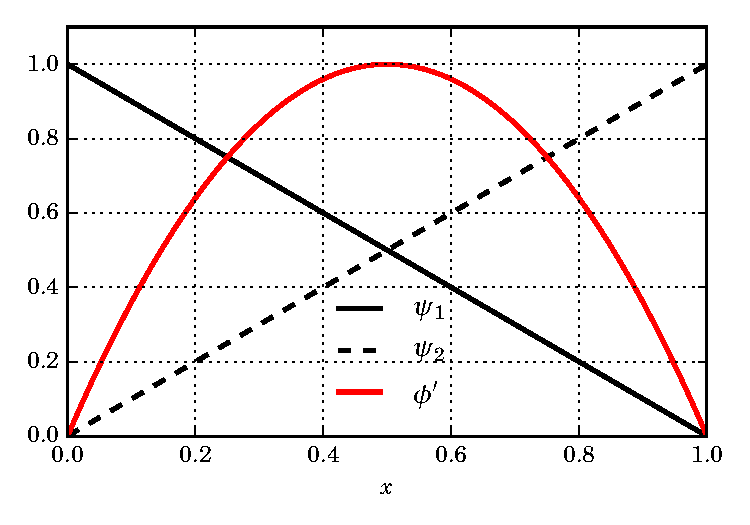
\includegraphics[width=\linewidth]{images/bubbles/bubble_new.pdf}
  \caption[One-dimensional bubble function]{The lowest order one-dimensional triangular element reference bubble function given by (\ref{bubble_function}) with $h_e = 1$.}
  \label{1d_bubble_image}
\end{figure}

\pythonexternal[label=bubble_2d_ftn_code, caption={Python code used to generate Figure \ref{2d_bubble_image}.}]{scripts/bubbles/bubble_2.py}

\begin{figure}
  \centering
    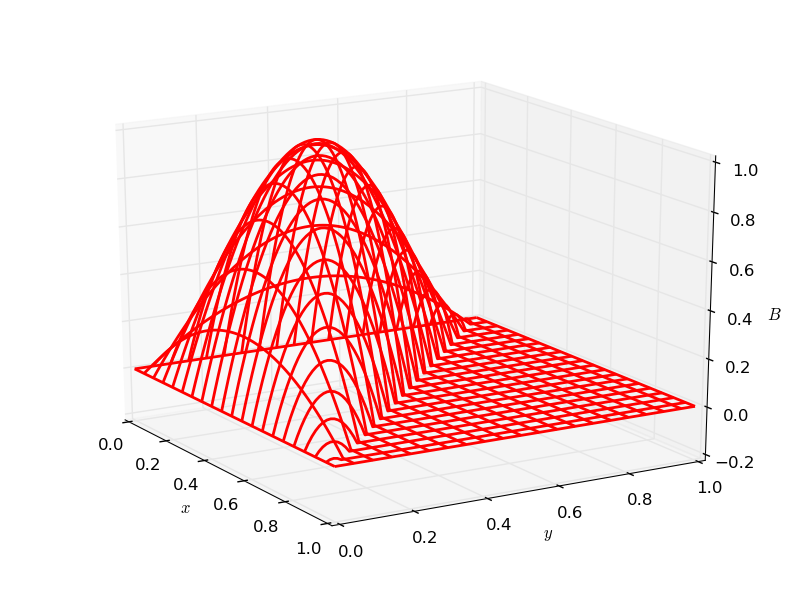
\includegraphics[width=\linewidth]{images/bubbles/2d_bubble.png}
  \caption[Two-dimensional bubble function]{The lowest order two-dimensional reference bubble function given by (\ref{2d_bubble_function}) with $h_x = h_y = 1$.}
  \label{2d_bubble_image}
\end{figure}

%===============================================================================

\section{Approximation of Green's function for $\Lu$ with bubbles}

Following the work of \citet{hughes_1995}, if $\phi'_j(x)$, $j \in 1,2,\ldots,N_b$ is a set of $N_b$ linearly independent bubble functions, a single element's unresolvable scales can be approximated -- in a process referred to as \index{Static condensation} \emph{static condensation} -- by linearly expanding $u'$ into $N_b$ nodes and $\bar{u}$ into $N_n$ nodes,
\begin{align}
  \label{bubble_u_approximation}
  u'(x) \approx u_h'(x) = \sum_{j=1}^{N_b} \phi_j'(x) u_j', \hspace{5mm} \bar{u}(x) \approx \bar{u}_h(x) = \sum_{j=1}^{N_n} \psi_j(x) \bar{u}_j,
\end{align}
where $u_j'$ is the coefficient associated with bubble function $j$ and $\bar{u}_j$ is the coefficient associated with a finite-element shape function $j$.

Fixing $w_k' = \phi_k'$ and inserting $u_h'(x)$ into (\ref{bubble_relation_2}),
\begin{align*}
  a(w_k', \bar{u}_h) + a(w_k',u_h')  &= (w_k',f) \\
  a(\phi_k', \bar{u}_h) + a\left( \phi_k', \sum_{j=1}^{N_b} \phi_j' u_j' \right)  &= (\phi_k',f) \\
  \left( \phi_k', \Lu \left( \sum_{j=1}^{N_b} \phi_j' u_j' \right) \right)  &= (\phi_k',f) - (\phi_k', \Lu \bar{u}_h) \\
  \left( \phi_k', \sum_{j=1}^{N_b} \Lu \phi_j' u_j' \right)  &= - \left( \phi_k', \Lu \bar{u}_h - f \right) \\
  \sum_{j=1}^{N_b} \left( \phi_k', \Lu \phi_j' \right) u_j'  &= - \left( \phi_k', \Lu \bar{u}_h - f \right) \\
  \sum_{j=1}^{N_b} a\left( \phi_k', \phi_j' \right) u_j'  &= - \left( \phi_k', \Lu \bar{u}_h - f \right),
\end{align*}
for $k = 1,2,\ldots,N_b$.  This implies that the $j$ nodal values of $u_h'(x)$ in (\ref{bubble_u_approximation}) are given by the linear system of equations
\begin{align*}
  u_j' &= - \sum_{k=1}^{N_b} a\left( \phi_j', \phi_k' \right)^{-1} \left( \phi_k'(x), \Lu \bar{u}_h(x) - f(x) \right),
\end{align*}
where $a\left( \phi_j', \phi_k' \right)^{-1}$ is the $jk$ component of the inverse of matrix $a\left( \phi_j', \phi_k' \right)$.  Inserting this into $u_h'(y)$ given by (\ref{bubble_u_approximation}),
{\footnotesize
\begin{align*}
  u_h'(y) &= \sum_{j=1}^{N_b} \phi_j'(y) u_j' \\
  &= \sum_{j=1}^{N_b} \phi_j'(y) \left[ - \sum_{k=1}^{N_b} a\left( \phi_j', \phi_k' \right)^{-1} \left( \phi_k'(x), \Lu \bar{u}_h(x) - f(x) \right) \right] \\
  &= -\sum_{j,k=1}^{N_b} \phi_j'(y) \left[ a\left( \phi_j', \phi_k' \right)^{-1} \left( \phi_k'(x), \Lu \bar{u}_h(x) - f(x) \right) \right] \\
  &= - \sum_{j,k=1}^{N_b} \int_{\Omega'} \phi_j'(y) \left[ a\left( \phi_j', \phi_k' \right)^{-1} \right] \phi_k'(x) \left(\Lu \bar{u}_h - f \right)(x) \d{\Omega_x'} \\
  &= - \int_{\Omega'} \left( \sum_{j,k=1}^{N_b} \phi_j'(y) \left[ a\left( \phi_j', \phi_k' \right)^{-1} \right] \phi_k'(x) \right) \left(\Lu \bar{u}_h - f \right)(x) \d{\Omega_x'} \\
  &= - \int_{\Omega'} \tilde{g}(x,y) \left(\Lu \bar{u}_h - f \right)(x) \d{\Omega_x'},
\end{align*}}
thus providing the Green's function approximation in (\ref{greens_ftn_prob})
\begin{align}
  \label{greens_ftn_approx}
  g(x,y) \approx \tilde{g}(x,y) = \sum_{j,k=1}^{N_b} \phi_j'(y) \left[ a\left( \phi_j', \phi_k' \right)^{-1} \right] \phi_k'(x).
\end{align}

Finally, inserting resolvable scale approximation $\bar{u}_h$ defined by (\ref{bubble_u_approximation}) and Green's function approximation (\ref{greens_ftn_approx}) into (\ref{bubble_relation_1_resolve}), we have
\begin{align}
  \label{bubble_relation_1_resolve_approx}
  (\bar{w}_h, \Lu \bar{u}_h) + (\Lu^* \bar{w}_h, \tilde{M}(\Lu\bar{u}_h - f)) &= (\bar{w}_h, f),
\end{align}
where
\begin{align*}
  M v(x) \approx \tilde{M} v(x) &= - \int_{\Omega'} \tilde{g}(x,y) v(x) \d{\Omega_x'},
\end{align*}
and the associated approximate bilinear form
\begin{align*}
  B(\bar{w}_h, \bar{u}_h; \tilde{g}) &= L(\bar{w}_h; \tilde{g}),
\end{align*}
where
\begin{align*}
  B(\bar{w}_h, \bar{u}_h; \tilde{g}) &= (\bar{w}_h, \Lu \bar{u}_h) + (\Lu^* \bar{w}_h, \tilde{M} \Lu\bar{u}_h) \\
  L(\bar{w}_h; \tilde{g}) &= (\Lu^* \bar{w}_h, \tilde{M}f) + (\bar{w}_h, f).
\end{align*}

%===============================================================================

\section{Stabilized methods} \label{ssn_stabilized_methods}

\index{Stabilization methods!Streamline-upwind/Petrov-Galerkin}
\index{Stabilization methods!Galerkin/least-squares}
\index{Stabilization methods!Subgrid-scale-model}
As described by \citet{hughes_1995} and \citet{codina_1992}, stabilized methods are \emph{generalized Galerkin methods} of the form
\begin{align}
  \label{generalized_form}
  (\bar{w}_h, \Lu \bar{u}_h) + (\mathbb{L} \bar{w}_h, \tau(\Lu\bar{u}_h - f)) &= (\bar{w}_h, f),
\end{align}
where operator $\mathbb{L}$ is a differential operator typically chosen from
\begin{align}
  \label{bubble_gls_operator}
  \mathbb{L} &= + \Lu && \text{Galerkin/least-squares (GLS)} \\
  \label{bubble_supg_operator}
  \mathbb{L} &= + \Lu_{\text{adv}} && \text{SUPG} \\
  \label{bubble_ssm_operator}
  \mathbb{L} &= - \Lu^* && \text{subgrid-scale model (SSM)}
\end{align}
where $\Lu_{\text{adv}}$ is the advective part of the operator $\Lu$.

Note that when using differential operator (\ref{bubble_ssm_operator}), stabilized form (\ref{generalized_form}) implies that $\tau = - \tilde{M} \approx -M$, and therefore the \index{Intrinsic-time parameter!General form} \emph{intrinsic-time} parameter $\tau$ approximates integral operator (\ref{subgrid_scale_integral}).  Equivalently,
\begin{align*}
  \tau \cdot \delta(y-x) = \tilde{g}(x,y) \approx g(x,y),
\end{align*}
and we can generate an explicit formula for $\tau$ by integrating over a single element $\Omega^e$,
{\footnotesize
\begin{align*}
  \int_{\Omega^e} \int_{\Omega^e} \tilde{g}(x,y) \d{\Omega^e_x} \d{\Omega^e_y} &= \int_{\Omega^e} \int_{\Omega^e} \tau \cdot \delta(y-x) \d{\Omega^e_x} \d{\Omega^e_y} = \tau h,
\end{align*}
\begin{align*}
  \implies \tau &= \frac{1}{h} \int_{\Omega^e} \int_{\Omega^e} \tilde{g}(x,y) \d{\Omega^e_x} \d{\Omega^e_y},
\end{align*}}
where $h$ is the element diameter.  Therefore, the parameter $\tau$ will depend both on the operator $\Lu$ and the basis chosen for Green's function approximation $\tilde{g}$ as evident by (\ref{greens_ftn_approx}).

For example, when $\Lu$ is the advective-diffusive operator $\Lu u = -\nabla \cdot \ranktwo{\sigma}(u) = -\nabla \cdot (k \nabla u - \rankone{a} u)$ and linear-Lagrange elements are used, the optimal expression for $\tau$ is the \emph{streamline upwind/Petrov-Galerkin} (SUPG) coefficient \citep{brooks_1982, hughes_1995}. 
\begin{align}
  \label{tau_supg}
  \tau_{\text{SUPG}} = \frac{h}{2|\rankone{a}|} \left( \coth(P_{\'e}) - \frac{1}{P_{\'e}} \right), \hspace{5mm} P_{\'e}  = \frac{h |\rankone{a}|}{2 \kappa},
\end{align}
where \index{Peclet@P\`eclet number!General form} $P_{\'e}$ is the element P\'eclet number and $\rankone{a}$ is the material velocity vector. 

On the other hand, if $\Lu$ is the diffusion-reaction operator $\Lu u = - \nabla \cdot \left( k \nabla u \right) + su$ with absorption coefficient $s \geq 0$, $P_{\'e}=0$ and $\tau$ is given by the coefficient \citep{hughes_1989}
\begin{align}
  \label{tau_dr}
  \tau_{\text{DR}} = \alpha \frac{h^2}{\kappa},
\end{align}
where $\alpha$ is a mesh-size-independent parameter dependent on the specific model used.  

When $\Lu$ is the advective-diffusion-reaction equation $\Lu u = - \nabla \cdot \left( k \nabla u \right) - \rankone{a} \cdot \nabla u + s u$, \citet{codina_1992} used the coefficient
\begin{align}
  \label{tau_adr}
  \tau_{\text{ADR}} = \frac{1}{\frac{4 \kappa}{h^2} + \frac{2 |\rankone{a}|}{h} + s},
\end{align}
to stabilize the formulation over a range of values for $s$ and $|\rankone{a}|$ using the space of linear Lagrange interpolation functions $\psi$.

Finally, when $\Lu$ is the Stokes operator $\Lu (\rankone{u},p) = -\nabla \cdot \ranktwo{\sigma}(\rankone{u},p) = -\nabla \cdot \left( 2\eta\ranktwo{\dot{\epsilon}}(\rankone{u}) - pI \right)$, $\tau$ has been found to be the coefficient \citep{hughes_1986}
\begin{align}
  \label{tau_stokes}
  \tau_{\text{S}} = \alpha \frac{h^2}{2\eta},
\end{align}
where the unknowns consist of the material velocity $\rankone{u}$ and pressure $p$ (see \S \ref{ssn_intro_stokes_2d}, \S \ref{ssn_intro_stokes_2d_slip}, and \S \ref{ssn_intro_stokes_3d}), and $\alpha > 0$ may or may not depend on the basis used for $\rankone{u}$.


%===============================================================================

\section{Diffusion-reaction problem}

\index{Linear differential equations!1D}
For an example, consider the steady-state advection-diffusion equation defined over the domain $\Omega \in [0,1]$
\begin{align}
  \label{bubble_example_1}
  \Lu u = - \kappa \totder[2]{u}{x} + s u = f, \hspace{4mm} u(0) = 1,\ u'(1) = 0,
\end{align}
with diffusion coefficient $\kappa$, absorption coefficient $s \geq 0$, and source term $f$ are constant throughout the domain.

\subsection{Bubble-enriched solution}

The bubble-function-enriched distributional form of the equation consists of finding $\hat{u} = \bar{u} + u'$ where $\bar{u} \in S_E^h \subset \mathcal{H}_E^1(\Omega)$ (see trial space (\ref{trial_space})) and $u' \in B_0^h \subset \mathcal{B}_0^2(\Omega)$ (see bubble space (\ref{bubble_space})) such that
\begin{align*}
  (\hat{\psi}, \Lu \hat{u}) &= (\hat{\psi}, f) \\
  -\kappa \int_{\Omega} \totder[2]{\hat{u}}{x} \hat{\psi} \d{\Omega} + s\int_{\Omega} \hat{u} \hat{\psi} \d{\Omega} &= \int_{\Omega} f \hat{\psi} \d{\Omega} \\
  \kappa \int_{\Omega} \totder{\hat{u}}{x} \totder{\hat{\psi}}{x} \d{\Omega} - \kappa \int_{\Gamma} \totder{\hat{u}}{x} \hat{\psi} \d{\Gamma} + s\int_{\Omega} \hat{u} \hat{\psi} \d{\Omega} &= \int_{\Omega} f \hat{\psi} \d{\Omega} \\
  \kappa \int_{\Omega} \totder{\hat{u}}{x} \totder{\hat{\psi}}{x} \d{\Omega} + s\int_{\Omega} \hat{u} \hat{\psi} \d{\Omega} &= \int_{\Omega} f \hat{\psi} \d{\Omega}.
\end{align*}
for all \emph{enriched} or \emph{augmented} test functions $\hat{\psi} = \psi + \phi$, where $\psi \in S_0^h \subset \mathcal{H}_E^1(\Omega)$ (see test space (\ref{test_space})) and $\phi \in B_0^h \subset \mathcal{B}_0^2(\Omega)$ (bubble space (\ref{bubble_space})).

\subsection{SSM-stabilized solution}

The subgrid-scale stabilized distributional form of the equation is derived by using subgrid-scale-model operator (\ref{bubble_ssm_operator}) and DR stability parameter (\ref{tau_dr}) within the general stabilized form (\ref{generalized_form}).  Thus, the stabilized problem consists of finding $\tilde{u} \in S_E^h \subset \mathcal{H}_E^1(\Omega)$ (see trial space (\ref{trial_space})) such that
\begin{align*}
  (\psi, \Lu \tilde{u}) - (\Lu^* \psi, \tau_{\text{DR}} (\Lu \tilde{u} - f)) &= (\psi, f),
\end{align*}
for all test functions $\psi \in S_0^h \subset \mathcal{H}_E^1(\Omega)$ (see test space (\ref{test_space})).  Using the fact that the diffusion-reaction operator (\ref{bubble_example_1}) is self adjoint, we have the bilinear form
\begin{align*}
  B(\tilde{u},\psi) &= L(\psi),
\end{align*}
where
{\footnotesize
\begin{align*} 
  B(u,\psi) &= \kappa \int_{\Omega} \totder{\tilde{u}}{x} \totder{\psi}{x} \d{\Omega} + s\int_{\Omega} \tilde{u} \psi \d{\Omega} - \frac{\alpha}{\kappa} \int_{\Omega} h^2 \left( \Lu^* \psi \right) \left( \Lu \tilde{u} \right) \d{\Omega} \\
  L(\psi) &= \int_{\Omega} f \psi \d{\Omega} - \frac{\alpha}{\kappa} \int_{\Omega} h^2 \Lu^* \psi f \d{\Omega}.
\end{align*}}

Note if linear Lagrange elements are used as a basis for $\tilde{u}$ and $\psi$, the diffusive terms with coefficient $\kappa$ in $\Lu \tilde{u}$ and $\Lu^* \psi$ will be zero.

\subsection{Analytic solution}

With the constants
\begin{align*}
  \kappa = \frac{1}{500}, \hspace{4mm} s = 1, \hspace{5mm} f = 0,
\end{align*}
the analytic solution to (\ref{bubble_example_1}) is 
$$u_{\text{a}}(x) = \frac{\exp\left(-10\sqrt{5}(x-2)\right) + \exp\left(10 \sqrt{5}x\right)}{1 + \exp\left(20\sqrt{5}\right)}.$$

Note that this is a heavily reaction-dominated problem, resulting in high gradients in the solution, referred to as a \index{Boundary layer} \emph{boundary layer}, near $x=0$.  The analytic solution is plotted against solutions determined with the standard Galerkin method with linear Lagrange elements $\psi$, quadratic-bubble-enriched linear Lagrange elements $\hat{\psi}$, and the SSM-stabilized formulation in Figure \ref{dr_analytic_image}, generated by Code Listing \ref{dr_analytic_code}.

\pythonexternal[label=dr_analytic_code, caption={FEniCS code used solve diffusion-reaction problem (\ref{bubble_example_1}).}]{scripts/bubbles/DR_analytic.py}

\begin{figure}
  \centering
    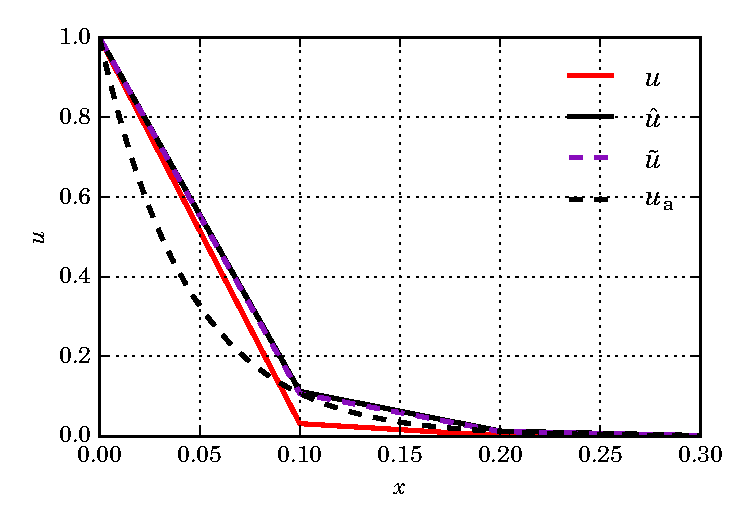
\includegraphics[width=\linewidth]{images/bubbles/DR_analytic_new.pdf}
  \caption[Diffusion-reaction stabilization example]{The analytic solution $u_{\text{a}}$ (black dashed) plotted against the unstabilized method solution $u$ (red), bubble-enriched solution $\hat{u}$ (dashed purple), and SSM-stabilized solution $\tilde{u}$ (black).  The parameter $\alpha = \frac{1}{15}$ was found by experimentation.}
  \label{dr_analytic_image}
\end{figure}

%===============================================================================

\section{Advection-diffusion-reaction example}

\index{Linear differential equations!1D}
Consider the model defined over the domain $\Omega \in [0,1]$
\begin{align}
  \label{bubble_example_2}
  \Lu u = -\kappa \totder[2]{u}{x} + d \totder{u}{x} + su = f, \hspace{4mm} u(0) = 0,\ u'(1) = 0,
\end{align}
where $\kappa$ is the diffusion coefficient, $d$ is the velocity of the material, $s \geq 0$ is an absorption coefficient, and $f$ is a source term.

\subsection{GLS-stabilized solution}

The Galerkin/least-squares  stabilized distributional form of the equation is derived by using GLS operator (\ref{bubble_gls_operator}) and ADR stability parameter (\ref{tau_adr}) within the general stabilized form (\ref{generalized_form}).  Thus, the stabilized problem consists of finding $\tilde{u} \in S_E^h \subset \mathcal{H}_E^1(\Omega)$ (see trial space (\ref{trial_space})) such that
\begin{align*}
  (\psi, \Lu \tilde{u}) + (\Lu \psi, \tau_{\text{ADR}} (\Lu \tilde{u} - f)) &= (\psi, f),
\end{align*}
for all test functions $\psi \in S_0^h \subset \mathcal{H}_E^1(\Omega)$ (see test space (\ref{test_space})).  Using ADR stability parameter (\ref{tau_adr}), we have the bilinear form
\begin{align*}
  B(\tilde{u},\psi) &= L(\psi),
\end{align*}
where
\begin{align*}
  B(\tilde{u}, \psi) = &+ \kappa \int_{\Omega} \totder{\tilde{u}}{x} \totder{\psi}{x} \d{\Omega} + d \int_{\Omega} \totder{\tilde{u}}{x} \psi \d{\Omega} + s\int_{\Omega} \tilde{u} \psi \d{\Omega} \\
  &+ \int_{\Omega} \tau_{\text{ADR}} \left( \Lu \psi \right) \left( \Lu \tilde{u} \right) \d{\Omega} \\
  L(\psi) = &+ \int_{\Omega} f \hat{\psi} \d{\Omega} + \int_{\Omega} \tau_{\text{ADR}} \Lu \psi f \d{\Omega}.
\end{align*}

Note if linear Lagrange elements are used as a basis for $\tilde{u}$ and $\psi$, the diffusive terms with coefficient $\kappa$ in $\Lu \tilde{u}$ and $\Lu \psi$ will be zero, and if $s = 0$, the GLS and SUPG operators given by (\ref{bubble_gls_operator}) and (\ref{bubble_supg_operator}), respectively, would in this case be identical \citep{hughes_1989}.

For an extreme example, we take
\begin{align*}
  \kappa = \frac{1}{100}, \hspace{4mm} d = 10, \hspace{4mm} s = 5,
\end{align*}
and
\begin{align*}
  f = \begin{cases}
        1000 & \text{ if } x = 0.5 \\
        0 & \text{ otherwise }
      \end{cases},
\end{align*}
resulting in an equation with low diffusivity that is heavily dominated by gradients of $u$ while advecting $u$ in the $+x$ direction.  Solutions determined with the standard Galerkin method with linear Lagrange elements $\psi$, quadratic-bubble-enriched linear Lagrange elements $\hat{\psi}$, and the GLS-stabilized formulation are depicted in Figure \ref{dr_extreme_image} and generated by Code Listing \ref{dr_extreme_code}.

\pythonexternal[label=dr_extreme_code, caption={FEniCS code used solve advection-diffusion-reaction problem (\ref{bubble_example_2}).}]{scripts/bubbles/ADR.py}

\begin{figure}
  \centering
    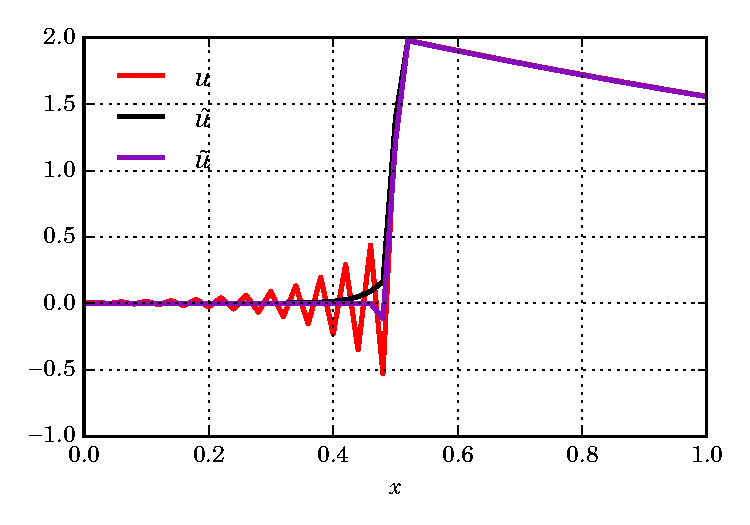
\includegraphics[width=\linewidth]{images/bubbles/extreme_new.pdf}
  \caption[Advection-diffusion-reaction stabilization example]{The unstabilized method solution $u$ (red), bubble-enriched solution $\hat{u}$ (black), and GLS-stabilized solution $\tilde{u}$ (purple) with identical mesh spacing.}
  \label{dr_extreme_image}
\end{figure}

%===============================================================================

\section{Stabilized Stokes equations} \label{ssn_intro_stokes_2d_slip_stab}

\index{Linear differential equations!2D}
\index{Stokes equations!Slip-friction}
\index{Nitsche method}
In this section we formulate a stabilized version of the slip-friction Stokes example described in \S \ref{ssn_intro_stokes_2d_slip} that circumvents inf-sup condition (\ref{inf_sup_condition}).  Recall that the Stokes equations for incompressible fluid over the domain $\Omega = [0,1] \times [0,1]$ are
\begin{align}
  \label{intro_stokes_stab_momentum}
  \Lu (\rankone{u}, p) = -\nabla \cdot \ranktwo{\sigma}(\rankone{u}, p) &= \rankone{f} &&\text{ in } \Omega \\
  \label{intro_stokes_stab_mass}
  \nabla \cdot \rankone{u} &= 0 &&\text{ in } \Omega,
\end{align}
where $\ranktwo{\sigma}(\rankone{u}, p) = 2\eta\ranktwo{\dot{\epsilon}} - pI$ is the Cauchy-stress tensor.  The boundary conditions considered here are of type Dirichlet and traction (Neumann),
\begin{align}
  \label{intro_stokes_stab_gD_N_S_D_slip}
  \rankone{u} \cdot \normal &= g_D = 0 &&\text{ on } \Gamma_N, \Gamma_S, \Gamma_D \\
  \label{intro_stokes_stab_gN_N_S_D_fric}
  \left( \ranktwo{\sigma} \cdot \normal \right)_{\Vert} &= \rankone{g_N} = -\beta \rankone{u} &&\text{ on } \Gamma_N, \Gamma_S, \Gamma_D \\
  \label{intro_stokes_stab_gD_E}
  \rankone{u} &= \rankone{g_D} = [-\sin(\pi y)\ 0]\T &&\text{ on } \Gamma_E \\
  \label{intro_stokes_stab_gN}
  \ranktwo{\sigma} \cdot \normal &= \rankone{g_N} = [g_{N_x}\ g_{N_y}]\T = \rankone{0} &&\text{ on } \Gamma_W,
\end{align}
where $\Gamma_E$, $\Gamma_W$, $\Gamma_N$, and $\Gamma_S$ are the East, West, North, and South boundaries, $\Gamma_D$ is the dolphin boundary (Figure \ref{intro_stokes_2d_nitsche_stab}) and $\normal$ is the outward-pointing normal vector to these faces.

It has been shown by \citet{hughes_1986} that the stabilized Galerkin approximate solution $(\rankone{u}, p)$ to Stokes system (\ref{intro_stokes_stab_momentum}, \ref{intro_stokes_stab_mass}) is given by solving the system
\begin{align}
  \label{stokes_stab_one}
  \begin{cases}
    \left( \rankone{\Phi}, \Lu (\rankone{u}, p) \right) = (\rankone{\Phi}, \rankone{f}), & \rankone{\Phi} \in \rankone{S_0^h}, \\
    \left( \xi, \nabla \cdot \rankone{u} \right) + \left( \nabla \xi, \tau_{\text{S}} \left( \Lu (\rankone{u}, p) - f \right) \right) = 0, & \xi \in M^h, 
  \end{cases}
\end{align}
where the coefficient $\alpha$ in $\tau_{\text{S}}$ given by (\ref{tau_stokes}) is constrained to obey $0 < \alpha < \alpha_0$, where the upper bound $\alpha_0$ depends on the basis used (the shape functions) for $\rankone{u}$ and $\rankone{\Phi}$.

A modification was made to (\ref{stokes_stab_one}) by \citet{hughes_1987} that allowed for discontinuous pressure spaces to be used.  The form for this model is given by
\begin{align}
  \label{stokes_stab_hughes_VII}
  B_{\text{VII}}(\rankone{u},p,\rankone{\Phi}, \xi) = L_{\text{VII}}(\rankone{\Phi}, \xi),
\end{align}
where
\begin{align}
  \label{stokes_stab_hughes_VII_B}
  B_{\text{VII}}(\rankone{u},p,\rankone{\Phi}, \xi) = &+ \left( \rankone{\Phi}, \Lu (\rankone{u}, p) \right) - \left( \xi, \nabla \cdot \rankone{u} \right) \notag \\
  &- \left( \Lu (\rankone{\Phi}, \xi), \tau_{\text{S}_{\Omega}} \Lu (\rankone{u}, p) \right) - \left( \llbracket \xi \rrbracket, \tau_{\text{S}_{\Gamma'}} \llbracket p \rrbracket \right)_{\Gamma'}, \\
  \label{stokes_stab_hughes_VII_L}
  L_{\text{VII}}(\rankone{\Phi}, \xi) = &+ ( \rankone{\Phi}, \rankone{f} ) - \left( \Lu (\rankone{\Phi}, \xi), \tau_{\text{S}_{\Omega}} f \right),
\end{align}
and 
\begin{align}
  \label{tau_stokes_VII}
  \tau_{\text{S}_{\Omega}} = \tau_{\text{S}} = \alpha \frac{h^2}{2\eta}, \hspace{10mm}
  \tau_{\text{S}_{\Gamma'}} = \zeta \frac{h^2}{2\eta}.
\end{align}
with constants $\alpha, \zeta \geq 0$ are dependent on the basis used for $\rankone{u}$ and $\rankone{\Phi}$.  Note that the notation $\llbracket \cdot \rrbracket$ denotes jump across interior edges, \ie across the $+$ and $-$ sides of an edge,
\begin{align*}
  \llbracket \psi \rrbracket = \psi^+ - \psi^-.
\end{align*}
Therefore, if a continuous basis is used for $p$ and $\xi$, $\zeta$ can be taken to be zero due to the fact that the jump terms in (\ref{stokes_stab_hughes_VII}) will have no effect.

An independent analysis from \citet{hughes_1987} was presented by \citet{douglas_1989} possessing a remarkably similar form, but where $\alpha$ and $\zeta$ were shown to be shape-independent.  This \emph{absolutely stabilized} model possesses the form
\begin{align}
  \label{stokes_stab_douglas}
  B_{\text{AS}}(\rankone{u},p,\rankone{\Phi}, \xi) = L_{\text{AS}}(\rankone{\Phi}, \xi),
\end{align}
where
\begin{align}
  \label{stokes_stab_douglas_B}
  B_{\text{AS}}(\rankone{u},p,\rankone{\Phi}, \xi) = &+ \left( \rankone{\Phi}, \Lu (\rankone{u}, p) \right) + \left( \xi, \nabla \cdot \rankone{u} \right) \notag \\
  &+ \left( \Lu (\rankone{\Phi}, \xi), \tau_{\text{S}_{\Omega}} \Lu (\rankone{u}, p) \right) + \left( \llbracket \xi \rrbracket, \tau_{\text{S}_{\Gamma'}} \llbracket p \rrbracket \right)_{\Gamma'}, \\
  \label{stokes_stab_douglas_L}
  L_{\text{AS}}(\rankone{\Phi}, \xi) = &+ ( \rankone{\Phi}, \rankone{f} ) + \left( \Lu (\rankone{\Phi}, \xi), \tau_{\text{S}_{\Omega}} f \right),
\end{align}
and utilizes the same coefficients $\tau_{\text{S}_{\Omega}}$ and $\tau_{\text{S}_{\Gamma'}}$ defined by (\ref{tau_stokes_VII}) with the difference that they possess only the single positivity constraint $\alpha, \zeta \geq 0$.  Note that the only difference between (\ref{stokes_stab_hughes_VII}) and (\ref{stokes_stab_douglas}) is the sign of the last two terms of bilinear forms (\ref{stokes_stab_hughes_VII_B}, \ref{stokes_stab_douglas_B}) and the last term of linear forms (\ref{stokes_stab_hughes_VII_L}, \ref{stokes_stab_douglas_L}).
  
The Galerkin/least-squares stabilized bilinear form for Dirichlet-traction-Stokes system (\ref{intro_stokes_stab_momentum}, \ref{intro_stokes_stab_mass}, \ref{intro_stokes_stab_gD_N_S_D_slip} -- \ref{intro_stokes_stab_gN}) are found identically to the formation of Nitsche variational form (\ref{intro_stokes_slip_var_form}); integration by parts of $(\rankone{\Phi}, \Lu (\rankone{u},p))$ and the addition of symmetric Nitsche terms, with the incorporation of the extra GLS terms of (\ref{stokes_stab_douglas}),

\begin{align}
  \label{intro_stokes_slip_stab_var_form}
  \mathcal{B}_{\Omega} + \mathcal{B}_{\Gamma_G} + \mathcal{B}_{\Gamma_G}^W + \mathcal{B}_{\Gamma_E} + \mathcal{B}_{\Gamma_E}^W + \mathcal{B}_{\Omega}^B + \mathcal{B}_{\Gamma'}^B = \mathcal{F} + \mathcal{F}^W + \mathcal{F}^B,
\end{align}
with individual terms
\begin{align*}
  \mathcal{B}_{\Omega} = &+ \int_{\Omega} \ranktwo{\sigma}(\rankone{u},p) : \nabla \rankone{\Phi} \d{\Omega} + \int_{\Omega} \left( \nabla \cdot \rankone{u} \right) \xi \d{\Omega} \\
  \mathcal{B}_{\Gamma_G} = &- \int_{\Gamma_G} \left( \normal \cdot \ranktwo{\sigma}(\rankone{u},p) \cdot \normal \right) \normal \cdot \rankone{\Phi} \d{\Gamma_G} + \int_{\Gamma_G} \beta \rankone{u} \cdot \rankone{\Phi} \d{\Gamma_G} \\
  \mathcal{B}_{\Gamma_G}^W = &- \int_{\Gamma_G} \left( \normal \cdot \ranktwo{\sigma}(\rankone{\Phi},\xi) \cdot \normal \right) \normal \cdot \rankone{u}  \d{\Gamma_G} + \gamma \int_{\Gamma_G} \frac{1}{h} \left( \rankone{u} \cdot \normal \right) \left( \rankone{\Phi} \cdot \normal \right) \d{\Gamma_G} \\
  \mathcal{B}_{\Gamma_E} = &- \int_{\Gamma_E} \ranktwo{\sigma}(\rankone{u},p) \cdot \normal \cdot \rankone{\Phi} \d{\Gamma_E} \\
  \mathcal{B}_{\Gamma_E}^W = &- \int_{\Gamma_E} \ranktwo{\sigma}(\rankone{\Phi},\xi) \cdot \normal \cdot \rankone{u} \d{\Gamma_E} + \gamma \int_{\Gamma_E} \frac{1}{h}  \left( \rankone{\Phi} \cdot \rankone{u} \right) \d{\Gamma_E} \\
  \mathcal{B}_{\Omega}^B = &+ \frac{\alpha}{2} \int_{\Omega} \frac{h^2}{\eta} \Lu(\rankone{\Phi},\xi) \Lu(\rankone{u},p) \d{\Omega} \\
  \mathcal{B}_{\Gamma'}^B = &+ \frac{\zeta}{2} \int_{\Gamma'} \frac{h^2}{\eta} \llbracket \xi \rrbracket \llbracket p \rrbracket \d{\Gamma'}
\end{align*}
and
\begin{align*}
  \mathcal{F} = &+ \int_{\Omega} \rankone{f} \cdot \rankone{\Phi} \d{\Omega} \\ 
  \mathcal{F}^W = &- \int_{\Gamma_G} \left( \normal \cdot \ranktwo{\sigma}(\rankone{\Phi},\xi) \cdot \normal \right) g_D \d{\Gamma_G} + \gamma \int_{\Gamma_G} \frac{1}{h} g_D \rankone{\Phi} \cdot \normal \d{\Gamma_G} \\
  &- \int_{\Gamma_E} \ranktwo{\sigma}(\rankone{\Phi},\xi) \cdot \normal \cdot \rankone{g_D} \d{\Gamma_E} + \gamma \int_{\Gamma_E} \frac{1}{h} \left( \rankone{\Phi} \cdot \rankone{g_D} \right) \d{\Gamma_E} \\
  \mathcal{F}^B = & +\frac{\alpha}{2} \int_{\Omega} \frac{h^2}{\eta} \Lu(\rankone{\Phi},\xi) f \d{\Omega}
\end{align*}
where $\Gamma_G = \Gamma_N \cup \Gamma_S \cup \Gamma_D$ is the entire slip-friction boundary, $h$ is the element diameter, and $\gamma > 0$ is an application-specific parameter normally derived by experimentation (see \S \ref{ssn_intro_stokes_2d_slip}).

The mixed variational formulation \index{Mixed methods} consistent with problem (\ref{intro_stokes_stab_momentum}, \ref{intro_stokes_stab_mass}, \ref{intro_stokes_stab_gD_N_S_D_slip} -- \ref{intro_stokes_stab_gN}) reads: find mixed approximation $\rankone{u}, p \in \left( \rankone{S_E^h} \subset \left( \mathcal{H}_E^1(\Omega) \right)^2 \right) \times \left( M^h \subset L^2(\Omega) \right)$ subject to (\ref{intro_stokes_slip_stab_var_form}) for all $\rankone{\Phi}, \xi \in \left(\rankone{S_0^h} \subset \left( \mathcal{H}_{E_0}^1(\Omega) \right)^2 \right) \times \left( M^h \subset L^2(\Omega) \right)$.

The velocity and pressure solutions to this problem using linear Lagrange elements for both $\rankone{u}$ and $p$ are depicted in Figure \ref{intro_stokes_2d_nitsche_stab}, and were generated by Code Listing \ref{intro_stokes_2d_nitsche_stab_code}.

\pythonexternal[label=intro_stokes_2d_nitsche_stab_code, caption={FEniCS solution to the 2D-Nitsche-stabilized-Stokes-slip-friction problem of \S \ref{ssn_intro_stokes_2d_slip_stab}.}]{scripts/fenics_intro/2D_stokes_nitsche_stabilized.py}

\begin{figure*}
  \centering
  \begin{minipage}[b]{0.60\linewidth}
    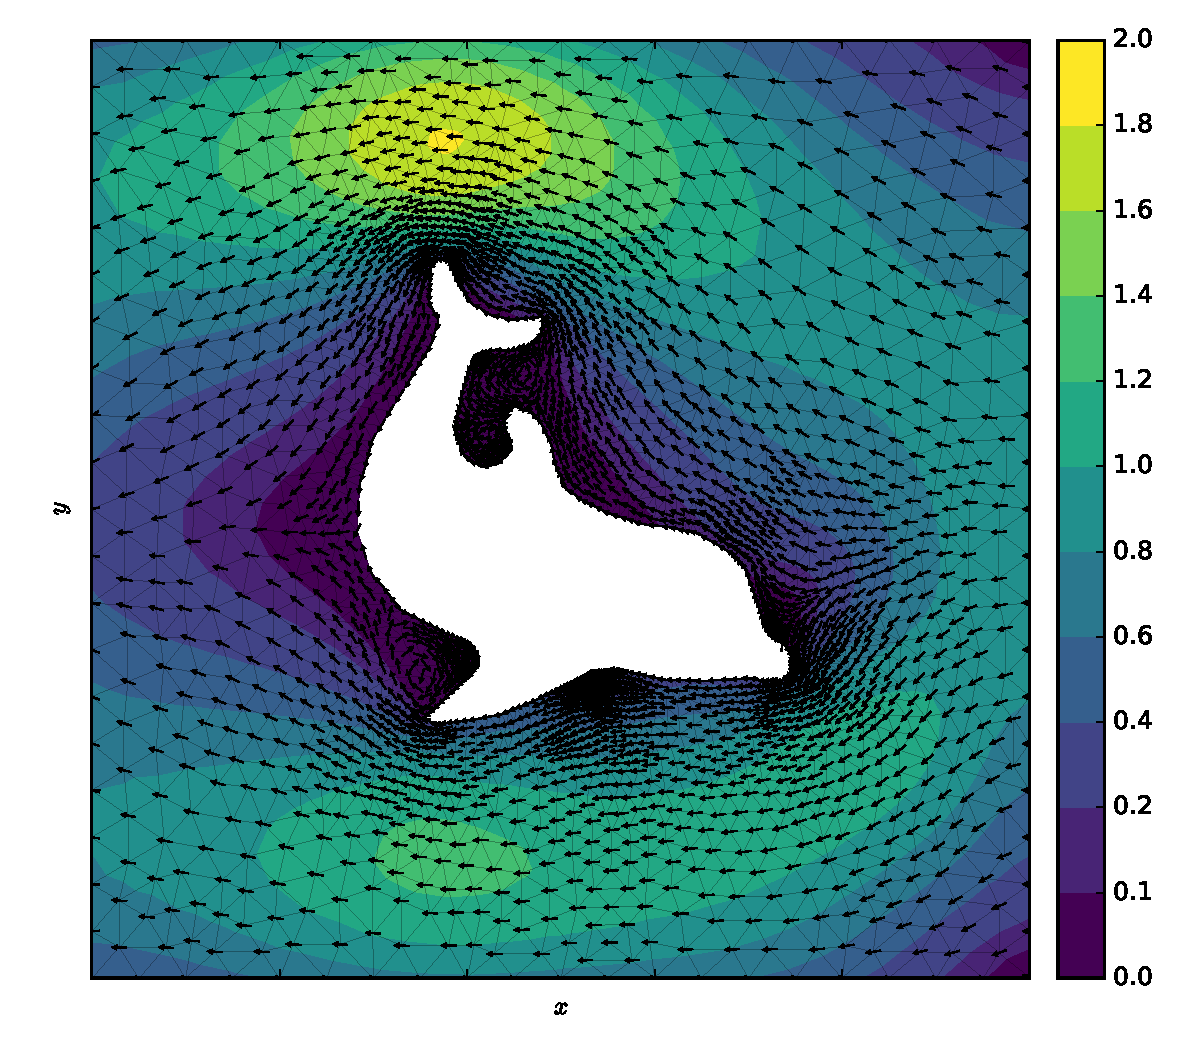
\includegraphics[width=\linewidth]{images/fenics_intro/2Dstokes_nitsche_u_stab.pdf}
  \end{minipage}
  \quad
  \begin{minipage}[b]{0.60\linewidth}
    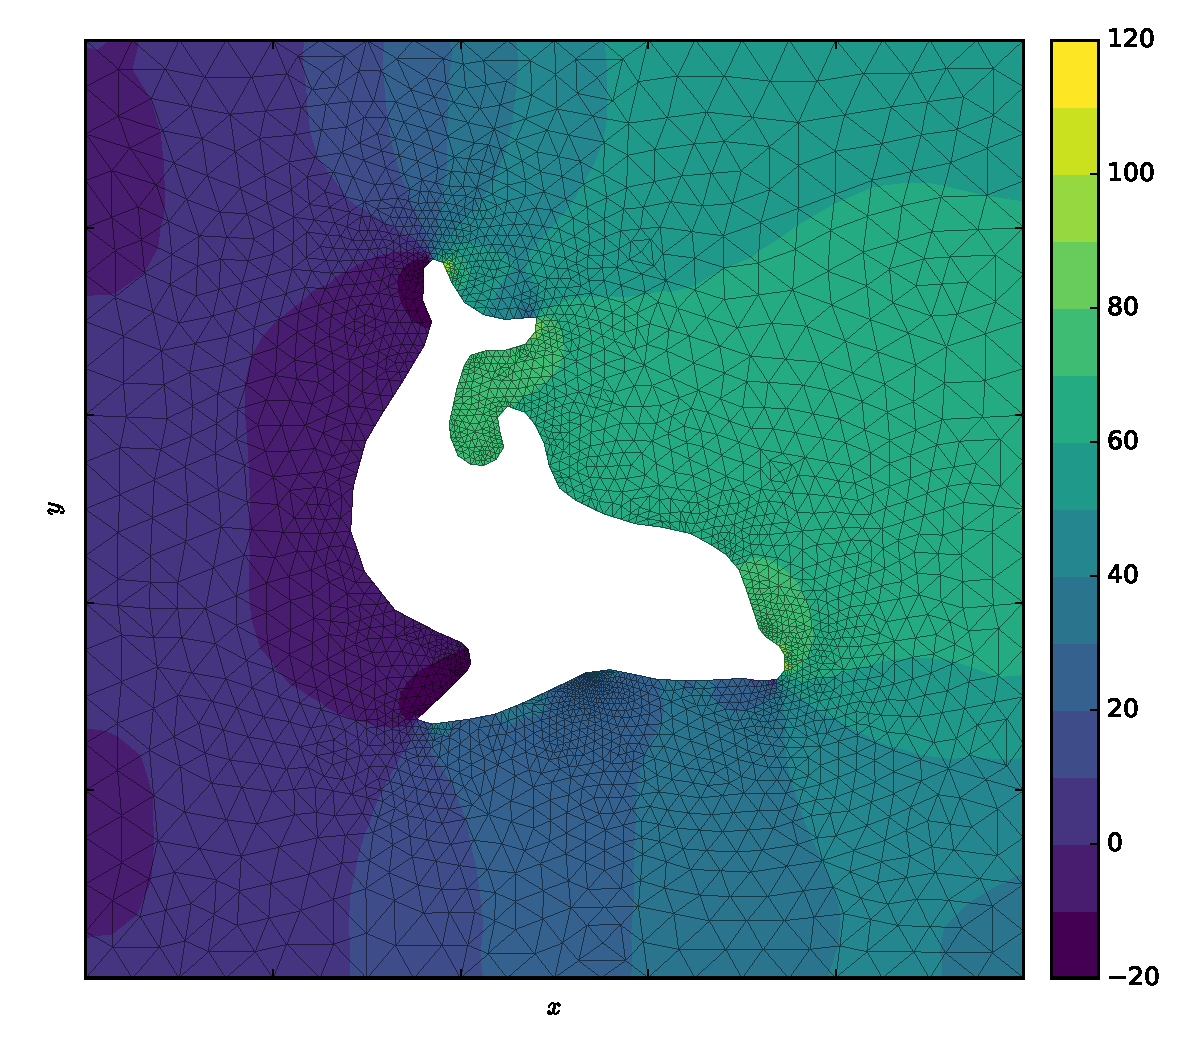
\includegraphics[width=\linewidth]{images/fenics_intro/2Dstokes_nitsche_p_stab.pdf}
  \end{minipage}
  \caption[GLS stabilized slip-friction Stokes example]{Galerkin/least-squares stabilized velocity field $\rankone{u}$ (top) and pressure $p$ (bottom) with $\alpha = 0.1$, $\zeta = 0$, $\beta = 10$, and $\gamma = 100$, utilizing continuous linear Lagrange elements for both $\rankone{u}$ and $p$ (referred to as P1 -- P1 approximation).}
  \label{intro_stokes_2d_nitsche_stab}
\end{figure*}
